%%%% IJCAI-ECAI-26 preprint
%%%%
%%%% BUILD:  pdflatex main && bibtex main && pdflatex main && pdflatex main
%%%% Needs ijcai26.sty and named.bst alongside this file (both gitignored --
%%%% they come from the official author kit and are not redistributed here).
%%%%
%%%% LENGTH: the main track allows seven pages plus at most two for
%%%% references, acknowledgements and statements. This draft is longer; the
%%%% sensitivity subsections are the first candidates for an appendix.

\documentclass{article}
\pdfpagewidth=8.5in
\pdfpageheight=11in

\usepackage{ijcai26}

% Use the postscript times font!
\usepackage{times}
\usepackage{soul}
\usepackage{url}
\usepackage[hidelinks]{hyperref}
\usepackage[utf8]{inputenc}
\usepackage[small]{caption}
\usepackage{graphicx}
\usepackage{amsmath}
\usepackage{amsthm}
\usepackage{booktabs}
\usepackage{algorithm}
\usepackage{algorithmic}
\usepackage{tikz}
\usetikzlibrary{arrows.meta,positioning,fit,backgrounds}
\usepackage[switch]{lineno}

% Comment out this line in the camera-ready submission
\linenumbers

\urlstyle{same}

% PDF Info Is REQUIRED.
% Please leave this \pdfinfo block untouched both for the submission and
% Camera Ready Copy. Do not include Title and Author information here.
\pdfinfo{
/TemplateVersion (IJCAI.2026.0)
}

\title{Cost-Derived Triage of Secret-Scanner Findings\\When the Credential Cannot Be Verified}

\author{
Grishma M\\
\emails
grishma.renuka@gmail.com
}

\begin{document}

\maketitle

\begin{abstract}
A secret scanner reports that a string in a repository looks like an API key. It
does not say whether the key works. The obvious way to find out---calling the
provider with the key---means authenticating with a credential belonging to
someone else, and we rule it out. This paper studies triage in the
\emph{no-direct-verification} setting: the hidden state is not merely unknown,
it is one we have decided not to resolve by the available means.

We model the finding as one of three hidden states (live, revoked, fake), price
five candidate actions in engineer-minutes, and select by minimising expected
cost. No threshold is tuned; the decision boundaries fall out of the cost
matrix. Against an idealised escalate-everything baseline, the cost-derived
policy saves $23.2\%$ of modelled engineer-minutes per finding while escalating
nothing. Every figure here is an expectation under our own cost model, not a
measurement of real triage work.

Three results were not designed in. First, the two free features we model cannot
distinguish a live key from a revoked one at all: both states carry identical
likelihoods on each, so their posterior ratio is invariant at $1.778$, which
also confines the agent to a one-dimensional slice of the belief simplex.
Second, escalation \emph{as a way of resolving the hidden state} is never
cost-optimal at any reachable belief: a perfect oracle is worth at most $15.03$
minutes there. Third, and least flattering, a policy that observes
\emph{nothing at all} already captures $21.2$ of the $23.2$ percentage points.
Joint sensitivity analysis over 40{,}000 sampled cost models shows the ordering
of these results is stable and the magnitudes are not.
\end{abstract}

\section{Introduction}

Secret scanners are widely deployed and reasonably good at what they do. What
they produce is a finding: \emph{this string, in this file, looks like a
credential of this type}. What they do not produce is the thing a responder
actually needs, which is whether the credential still works.

The gap matters because the available actions differ enormously in cost. Doing
nothing about a live key risks whatever sits behind it. Revoking immediately is
cheap and certain, and breaks anything still using it. Rotating safely avoids
the outage and costs a deploy cycle. Handing the finding to a person is reliable
and spends the scarcest resource in the organisation. The right choice depends
on a hidden state, and the standard method for resolving that state---issuing a
request with the found credential---is not one we are willing to use against a
third party's account.

That constraint is the origin of the problem we study. It is our choice, not a
consensus position: three practitioners told us, unprompted, to simply try the
key. We keep it, and treat it as the paper's most load-bearing assumption.

\paragraph{Contributions.}
\begin{enumerate}
\item A decision-theoretic formulation of secret-scanner triage in which the
decision boundaries are \emph{derived} from a cost matrix rather than tuned. On
the slice of the simplex the agent can occupy, the derived boundary sits at
$P(\text{live}) = 0.066$ rather than near the $0.5$ an engineer would pick by
instinct.
\item A structural result: the two free features we model cannot separate live
from revoked keys, because both states carry identical likelihoods on each.
Given conditional independence this is arithmetic rather than an empirical
claim, and it is a property of the features chosen, not of repository evidence
in general.
\item A parametric bound on escalation: a perfect oracle is worth at most
$15.03$ minutes at any reachable belief, so escalation cannot be justified on
information-gathering grounds whenever human triage overhead exceeds that. This
bounds a human acting as a state oracle; it says nothing about a human who
supplies authority or organisational context.
\item A closed-world comparison showing that most of the improvement over the
baseline comes from the cost structure rather than from the belief model, and
that hand-picked thresholds respond non-monotonically to a prior we cannot pin
down.
\item A joint sensitivity study over 40{,}000 sampled cost and evidence models,
identifying which conclusions are robust and which are artefacts of point
estimates.
\end{enumerate}

\section{Related Work}

\paragraph{Detector precision is not a constant.}
A nine-tool comparison~\cite{basak2023comparative} reports precision of about
$75\%$ for GitHub's scanner, $46\%$ for Gitleaks, and below $7\%$ for five of
the nine, attributing the spread to over-broad regular expressions and entropy
scoring. There is therefore no such thing as \emph{the} base rate of true
positives; it is a property of which detector fired. We assume GitHub's scanner
throughout, and note that assuming a weaker detector would change the problem
from ``what should be done about this key'' to ``is this junk''.

\paragraph{Credential lifetime.}
GitGuardian~\cite{gitguardian2026} reports that roughly $64\%$ of credentials
valid in 2022 were still valid in January 2026. This is a vendor figure and we
treat it as a hypothesis, but it points the opposite way to intuition: commit
age is weak evidence that a key is dead.

\paragraph{Classification of secrets with language models.}
Recent work~\cite{islam2025secretbreach} reports GPT-4o at $93.29\%$ precision
few-shot for deciding whether a string \emph{is} a secret. This is the obvious
alternative technology and answers a different question: it improves detection
and says nothing about whether a detected credential is live, which is the axis
our decision turns on.

\paragraph{Decision theory and the value of information.}
The formulation here is expected-cost minimisation with pre-posterior analysis,
which is classical~\cite{raiffa1961applied,howard1966voi}. Deriving a decision
threshold from a cost matrix rather than tuning it is the central move of
cost-sensitive learning~\cite{elkan2001foundations,domingos1999metacost}, and
the buy-evidence-then-decide structure of our \textsc{investigate} action is
test-cost-sensitive learning~\cite{turney2000types}. The sequential formulation
we defer to in Section~\ref{sec:limitations} is a
POMDP~\cite{smallwood1973optimal,kaelbling1998pomdp}. Our contribution is not
the machinery but the instance: a domain where the machinery produces
predominantly negative results, and where we can say why.

\paragraph{Analyst load.}
The cost of human attention is the quantity our escalation result turns on.
Qualitative work on security operations~\cite{alahmadi2022falsepositives}
documents analysts discarding the majority of alerts under load, which is
evidence against our escalate-everything baseline being what teams actually run.

\paragraph{Revocation is solved for a different credential format.}
A practitioner observed during our discussion phase that a certificate carries a
CRL distribution point---a pointer to its own revocation list---so
live-versus-revoked is answered by the credential itself. Public-key
infrastructure solved decades ago the exact problem that motivates this paper.
An API key has no equivalent. \textbf{Our central difficulty is a property of
API keys specifically, not of leaked credentials in general.}

\section{Problem Formulation}

\subsection{Input and hidden state}

The agent observes one scanner finding: a string in a repository matching a
known key format. The hidden state $s$ is one of

\begin{itemize}
\item \textbf{live} --- the credential still authenticates;
\item \textbf{revoked} --- it authenticated once and no longer does;
\item \textbf{fake} --- hard-coded by a developer, never authenticated.
\end{itemize}

We scope to a single provider, OpenAI, and to project keys. This collapses a
fourth state that exists elsewhere: Stripe issues distinguishable test keys,
OpenAI does not. The trade was deliberate---we gave up a hidden state to gain a
probe whose response shape is documented~\cite{openai2026admin}.

Only the first state carries the exposure risk we price. The other two do not,
though ``harmless'' would be too strong: a revoked key still has audit
implications and may have been reused elsewhere.

\subsection{Actions}

\begin{table}[t]
\centering
\begin{tabular}{ll}
\toprule
\textbf{Action} & \textbf{What it does} \\
\midrule
Dismiss & Nothing. The finding is closed. \\
Investigate & Buy evidence, then decide again. \\
Escalate & Hand the decision to a human. \\
Revoke now & Kill the key; accept the outage. \\
Rotate safely & Replace, migrate, verify, revoke. \\
\bottomrule
\end{tabular}
\caption{The five candidate actions. Section~\ref{sec:notterminal} argues only
three are terminal.}
\label{tab:actions}
\end{table}

\begin{figure}[t]
\centering
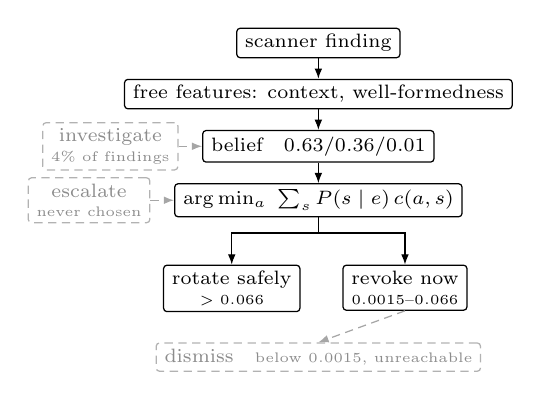
\begin{tikzpicture}[
  font=\scriptsize,
  box/.style={draw, rounded corners=1.2pt, line width=.45pt, inner xsep=3pt,
              inner ysep=2.2pt, align=center},
  dead/.style={box, draw=black!30, text=black!45, densely dashed},
  ar/.style={-{Latex[length=1.3mm]}, line width=.45pt},
  arw/.style={-{Latex[length=1.3mm]}, line width=.45pt, draw=black!35,
              densely dashed},
  node distance=2.6mm,
]
\node[box] (f) {scanner finding};
\node[box, below=of f] (e) {free features: context, well-formedness};
\node[box, below=of e] (b) {belief \; $0.63 / 0.36 / 0.01$};
\node[box, below=of b] (p) {$\arg\min_{a}\ \sum_{s} P(s\mid e)\, c(a,s)$};

\node[box, below=6mm of p, xshift=-11mm] (rot) {rotate safely\\[-1pt]{\tiny $>0.066$}};
\node[box, below=6mm of p, xshift=11mm]  (rev) {revoke now\\[-1pt]{\tiny $0.0015$--$0.066$}};
\node[dead, below=4mm of rev, xshift=-11mm] (dis) {dismiss \; {\tiny below $0.0015$, unreachable}};

\node[dead, left=3mm of b.west] (iv) {investigate\\[-1pt]{\tiny 4\% of findings}};
\node[dead, left=3mm of p.west] (es) {escalate\\[-1pt]{\tiny never chosen}};

\draw[ar] (f) -- (e);
\draw[ar] (e) -- (b);
\draw[ar] (b) -- (p);
\draw[ar] (p.south) -- ++(0,-2mm) -| (rot.north);
\draw[ar] (p.south) -- ++(0,-2mm) -| (rev.north);
\draw[arw] (rev.south) -- (dis.north);
\draw[arw] (iv) -- (b);
\draw[arw] (es) -- (p);
\end{tikzpicture}
\caption{The agent. Two free features produce a belief; the cheapest terminal
action follows from the cost matrix. Dashed paths are those the policy takes
rarely or never: \textsc{investigate} fires on $4\%$ of findings,
\textsc{escalate} on none, and \textsc{dismiss} on no belief the agent can
reach. That two of five actions go unused is a result, not an omission.}
\label{fig:pipeline}
\end{figure}

Revoke-now and rotate-safely are kept separate because leaving a system broken
in order to be safe is not automatically correct, and a model that cannot
express the difference cannot inform the choice. This separation is justified a
second time in Section~\ref{sec:regimes}, from an argument we did not
anticipate.

\subsection{Baseline and objective}

Our baseline is an \textbf{idealised escalate-everything policy}: every finding
goes to a person, and that person resolves it correctly. We do not claim this is
what teams do today---real pipelines allowlist known fixtures, auto-dismiss, and
route by pattern before any human sees an alert. It is a deliberately favourable
comparator, chosen because it makes the argument clean: \textbf{the baseline is
never wrong about the hidden state.} There is therefore no accuracy for an
automated method to win, and the only remaining axis is cost.

\begin{quote}
\textbf{Objective.} Does a probabilistic, cost-aware policy reach the same
decisions as escalate-everything while spending fewer human interruptions---and
under what conditions does it stop doing so?
\end{quote}

The second clause carries most of the weight. A policy that wins under every
assumption we could vary would be evidence the comparison was built badly.

\section{Model}

\subsection{Prior}

We \emph{construct} a traceable prior from two external estimates rather than
estimating one from representative data. GitHub's scanner reports about $75\%$
precision; of real credentials, about $64\%$ are still valid. This gives
\[
P(\text{live}) = 0.48,\quad
P(\text{revoked}) = 0.27,\quad
P(\text{fake}) = 0.25.
\]

Its virtue is traceability, not accuracy. Two caveats belong here rather than in
the limitations. The $0.64$ describes credentials known valid in 2022 and still
valid in 2026, which is not the population a scanner reports today; and detector
precision counts strings that are not credentials at all, whereas our
\emph{fake} state is a real-format string that never authenticated. We merge
those populations and its likelihood row is a guess for both.

\subsection{Evidence}

Two features are free---readable from the repository at no cost---and one must
be purchased.

\textbf{Placeholder context} (placeholder / neutral / production), from the file
path, variable name, and commit message. \textbf{Well-formedness} (well-formed /
malformed), whether the string matches the published format.
\textbf{\texttt{last\_used\_at}} (recent / old / null), a timestamp obtained by
asking \emph{our own} account about the key through the provider's admin API.
This never involves authenticating \emph{as} the suspect key.

\paragraph{Conditional independence.}
We assume features are conditionally independent given the hidden state, so that
$P(c,f,r \mid s) = P(c \mid s)P(f \mid s)P(r \mid s)$. This licenses the
multiplication in every posterior below and makes
Section~\ref{sec:invariance}'s result follow from the rows of
Table~\ref{tab:likelihoods} rather than from a joint distribution we never
specify. It is an assumption of convenience and plainly imperfect: a string that
reads as a placeholder from its path is more likely to be malformed than the
product suggests.

\begin{table}[t]
\centering
\footnotesize
\setlength{\tabcolsep}{4pt}
\begin{tabular}{lccc}
\toprule
\textbf{Feature} & \textbf{live} & \textbf{revoked} & \textbf{fake} \\
\midrule
Context: pl./ne./pr. & .10/.30/.60 & .10/.30/.60 & .70/.25/.05 \\
Form: well/mal & .99/.01 & .99/.01 & .40/.60 \\
\texttt{last\_used}: rec./old/null & .60/.20/.20 & .02/.78/.20 & .01/.04/.95 \\
\bottomrule
\end{tabular}
\caption{$P(e \mid s)$. Live and revoked are identical on both free features.}
\label{tab:likelihoods}
\end{table}

\subsection{A structural consequence}
\label{sec:invariance}

Note the first two rows of Table~\ref{tab:likelihoods}. \textbf{Live and revoked
carry identical likelihoods on both free features.} This is not a modelling
convenience; it reflects that nothing visible inside a repository distinguishes
a key that works from one that was turned off. Identical rows cancel in the
update, so the posterior ratio is invariant:
\[
\frac{P(\text{live} \mid e_{\text{free}})}{P(\text{revoked} \mid e_{\text{free}})}
= \frac{0.48}{0.27} = 1.778 \quad \text{for every } e_{\text{free}}.
\]

On our worked case the posterior is $0.6329 / 0.3560 / 0.0111$, and
$0.6329/0.3560 = 1.778$ to four decimal places. The free evidence does one job
excellently---it collapses \emph{fake} from $0.25$ to $0.011$---and the other
not at all.

\textbf{Neither of these two features can move the ratio that matters}, at any
value, in any combination. We state it narrowly on purpose: this is a property
of the two static text features we chose, not of repository evidence in general.
Section~\ref{sec:limitations} names two we did not model---repository visibility
and commit semantics---that would plausibly separate the two states, and the
claim is safest read as applying to findings in private repositories.

\subsection{Costs}

Fifteen cells built from nine components, in engineer-minutes, so a practitioner
can dispute a component rather than a cell. Components: revoke 2, issue a new
key 10, run the probe 3, human attention 30, find the consumers 30 (documented)
or 480 (undocumented), deploy 60, verify 10, production outage 240.

\begin{table}[t]
\centering
\begin{tabular}{lrrr}
\toprule
& \textbf{live} & \textbf{revoked} & \textbf{fake} \\
\midrule
Dismiss & \textbf{2400} & 2 & 2 \\
Investigate & 3 & 3 & 3 \\
Escalate & 142 & 32 & 32 \\
Revoke now & 332 & 2 & 5 \\
Rotate safely & \textbf{112} & 30 & 20 \\
\bottomrule
\end{tabular}
\caption{The cost matrix, engineer-minutes. The live column is exact component
sums.}
\label{tab:costs}
\end{table}

Rotate-safely on live is $10+30+60+10+2 = 112$; revoke-now is the same hunt and
deploy plus the outage, $2+240+30+60 = 332$. Escalate is defined throughout as
$30 + \min_a c(a,s)$---human attention plus whatever that human then correctly
does---giving $142/32/32$.

Three cells are direct estimates with no component decomposition: rotating a
revoked key (30) or a fake one (20), and revoking a fake one (5). The
rotate-on-fake figure is the cost of beginning a rotation and discovering there
is nothing to rotate. It is load-bearing: Section~\ref{sec:onecell} shows that
setting it to zero makes the belief model worth exactly nothing.

\subsection{Investigate is not a terminal action}
\label{sec:notterminal}

The investigate row is not the same kind of number as the other four. The others
are what an action \emph{costs}; this one is an entry fee. Investigate does not
close the case---it buys an answer and returns the decision to the agent.
Placing 3 into the minimisation alongside the rest would make it win at every
belief, and the agent would probe forever without acting.

We therefore minimise over the four \textbf{terminal} actions, and compare
investigate separately by whether the expected value of the information exceeds
its price. The general rule: \emph{a sequence of steps may be collapsed into a
single action when no observation inside the sequence changes what is done
next.} Rotate-safely observes but does not branch, so it collapses. Investigate
exists only to branch, so it cannot.

\section{Policy}

\subsection{Selection}

\begin{equation}
a^\star = \arg\min_{a \in \mathcal{A}_{\text{terminal}}}
\sum_{s} P(s \mid e)\, c(a, s)
\end{equation}

No threshold appears in this expression. Thresholds are a consequence of it.

\subsection{The derived regimes}
\label{sec:regimes}

With three states, $P(\text{live})$ alone does not determine the cheapest
action---the split of the remaining mass between revoked and fake matters too. A
boundary is therefore only meaningful relative to a path through the simplex,
and Section~\ref{sec:invariance} tells us which: the free features lock
$P(\text{live}):P(\text{revoked})$ at $1.778$, so the agent walks one line and
never leaves it. All boundaries below are measured on that line.

\begin{figure}[t]
\centering
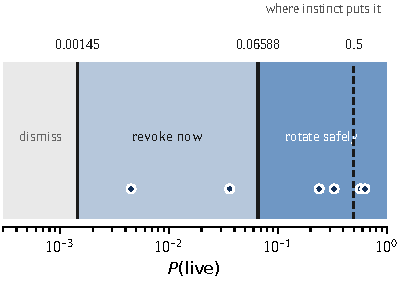
\includegraphics[width=\columnwidth]{figures/regimes.pdf}
\caption{Decision regimes on the reachable line, and the six posteriors the
agent can actually hold (dots). The derived boundary between revoking and
rotating sits at $0.066$; the dashed line at $0.5$ is where an engineer sets it
by instinct. Everything between the two is dismissed by the naive rule and
rotated by ours.}
\label{fig:regimes}
\end{figure}

\textbf{The boundary is at $0.066$, not $0.5$.} An engineer building this by
instinct places the line at ``more likely than not'' and dismisses findings this
model rotates; Section~\ref{sec:results} measures what that costs.

And \textbf{revoke-now owns an entire regime on its own}. We introduced it
because outages are not automatically acceptable; the arithmetic justifies it
from a different direction, and a model with a single remediation action would
never have exposed that region.

\subsection{A bound on escalation}
\label{sec:escalation}

At each belief we compute the value of perfect information---the cost saved by
an oracle revealing the true state. This upper-bounds what a human who
\emph{only resolves the hidden state} could be worth.

Over the whole simplex the maximum is $24.78$ minutes, but that maximiser lies
at $b \approx (0.12, 0.88, 0.00)$, which the agent cannot reach. Over the six
beliefs it can hold,
\begin{equation}
\max_{b \in \mathcal{B}_{\text{reachable}}} \mathrm{VPI}(b) = 15.03 \text{ min.}
\end{equation}

So escalation is dominated whenever a human costs more than $15.03$ minutes. At
our assumed 30 it loses comfortably; at the 10--15 minutes a dedicated triage
analyst might cost, it does not. \textbf{This is a parametric result, not a
structural one}, and it bounds only the informational value of a human. A person
supplying authority to act on another team's credential is not bounded by any
VPI calculation.

\subsection{Uncertainty is not the trigger}

It is natural to escalate when confused. We tested the most confused belief
available, $(1/3,1/3,1/3)$ at $1.585$ bits. Rotate-safely costs $54.00$;
escalate costs $68.67$.

\textbf{Entropy measures confusion. It does not measure whether the confusion is
expensive.} Two roads at a fork are maximally uncertain and the choice does not
matter; a fire alarm that is probably faulty is barely uncertain and urgently
needs a person. Entropy retains a role---counting the bits a probe removes---but
the escalation trigger is the cost of being wrong.

\subsection{When to buy the probe}

Three context values and two form values give exactly \textbf{six} reachable
posteriors, small enough to enumerate rather than sample.

\begin{table}[t]
\centering
\small
\begin{tabular}{llrrlr}
\toprule
\textbf{Context} & \textbf{Form} & $P(\text{seen})$ & $P(\text{live})$ & \textbf{Act} & \textbf{EVSI} \\
\midrule
placeholder & well & .1442 & .3294 & rotate & 0.00 \\
placeholder & mal & .1057 & .0045 & revoke & 1.40 \\
neutral & well & .2477 & .5754 & rotate & 0.00 \\
neutral & mal & .0398 & .0362 & revoke & \textbf{5.21} \\
production & well & .4505 & .6329 & rotate & 0.00 \\
production & mal & .0120 & .2400 & rotate & 0.00 \\
\bottomrule
\end{tabular}
\caption{Value of the probe at every belief the agent can hold.}
\label{tab:evsi}
\end{table}

At the four beliefs where rotate-safely is already optimal, every probe outcome
leaves it optimal, so the information is worth exactly nothing. Value
concentrates at the two beliefs near a boundary.

Because EVSI takes only \textbf{two} non-zero values, the probe's price selects
one of three regimes rather than tuning behaviour continuously: below $1.40$ it
is bought on $14.55\%$ of findings, between $1.40$ and $5.21$ on $3.98\%$, and
above $5.21$ never. We initially priced it at ten minutes by guesswork; a
practitioner who uses it offered roughly one minute, and a second warned against
concluding anything from a single response. One minute per call, three calls,
gives three.

Two things follow. \textbf{Investigation becomes rational at $5.21$ minutes},
which is a property of the cost matrix rather than of the probe. And \textbf{it
never becomes important}: even at half a minute the aggregate saving is $0.283$
minutes per finding, four tenths of one percent. Information here is sometimes
worth buying and never worth much, and those are separate facts.

\section{Simulation Study}

Six policies on identical findings: the \textbf{baseline} (escalate every
finding); \textbf{P0} (act on the prior, observe nothing); \textbf{P1} (free
evidence, hand-picked thresholds---dismiss below $0.05$, revoke below $0.5$,
else rotate---over all four terminal actions); \textbf{P1-trunc} (the same
$0.5$ threshold over $\{$rotate, dismiss$\}$ only); \textbf{P2} (free evidence,
minimise expected cost); \textbf{P3} (P2 plus the probe when EVSI exceeds its
price).

P1 is the comparison that matters: hand-picked thresholds, but the same
information and actions available to P2, so it isolates \emph{where the
boundaries came from} and nothing else. P1-trunc is an earlier version of that
comparison which also restricted the action set; we report it because it
produces a dramatic result for the wrong reason.

Expected cost is computed in closed form over all 54 possible worlds and carries
no sampling error. Realised cost is measured on 40 cases drawn once with a fixed
seed and frozen thereafter.

\subsection{Why the study is a simulation, not an experiment}

The obvious alternative is SecretBench~\cite{basak2023secretbench}, a labelled
corpus of 97{,}479 candidate secrets, 15{,}084 confirmed real. We cite it and do
not use it, for a specific reason.

\textbf{SecretBench labels whether a string is a secret. It does not label
whether that secret still works.} Its fields would ground our \emph{fake} state,
the $0.25$ of prior mass assigned to it, and both free feature rows. There is no
field for live versus revoked---the axis this paper turns on. Fitting to it
would sharpen the half of the model that already works and leave the half that
matters untouched.

We record the gap as evidence rather than an obstacle. \textbf{The largest
public corpus of real leaked credentials does not record whether they still
authenticate}, and the reason is the one that motivates this paper: establishing
it would mean testing each key against its provider. The label is missing from
the dataset for precisely the reason the state is hidden from our agent.

\section{Results}
\label{sec:results}

\begin{table}[t]
\centering
\small
\begin{tabular}{llrrr}
\toprule
& \textbf{Policy} & \textbf{Cost} & \textbf{vs base} & \textbf{$\neq$ P0} \\
\midrule
base & escalate all & 84.80 & --- & --- \\
P0 & prior only & 66.86 & $-21.2\%$ & --- \\
P1 & hand-picked, 4 acts & 77.79 & $-8.3\%$ & 14.55\% \\
P1-t & hand-picked, 2 acts & 181.78 & $\mathbf{+114.4\%}$ & 14.55\% \\
P2 & cost-derived & 65.11 & $\mathbf{-23.2\%}$ & \textbf{14.55\%} \\
P3 & P2 + probe & 65.03 & $-23.3\%$ & 10.57\% \\
\bottomrule
\end{tabular}
\caption{Exact expected cost per finding. The last column is the share of
findings on which the policy chooses differently from P0's constant
``rotate safely''.}
\label{tab:main}
\end{table}

On the 40 frozen cases: baseline 2820 minutes, P2 2018, a $28.4\%$ saving. That
draw contains 14 live keys out of 40, a live share of $0.35$ against a prior of
$0.48$, so the sampled and exact figures are not interchangeable.

\subsection{The cost structure does the work}

P0 observes nothing whatsoever. It knows the base rates, concludes rotate-safely
is cheapest in expectation, and applies it to every finding. It beats the
baseline by $21.2\%$. The full belief model reaches $23.2\%$. \textbf{The
evidence is worth $1.75$ minutes per finding, and the remaining twenty-one
points come from a single decision: stop asking a human.} It does change the
action on $14.55\%$ of findings---it is not inert---but the action it changes to
is cheap enough that the aggregate barely moves.

The mechanism is that rotate-safely costs $112/30/20$: it is nearly state-blind
and tolerable whichever state obtains. When a hedge that good is available,
identifying the state buys very little. This is the EVSI result one level up.

\subsection{What hand-picked thresholds actually cost}

An earlier version of this comparison reported that the naive $0.5$ threshold
costs more than twice the baseline, and treated that as the strongest argument
for deriving boundaries. \textbf{That comparison was confounded.} P1-trunc
changes two things at once: it moves the boundary to $0.5$ \emph{and} restricts
the action set, withholding revoke-now. Holding the threshold fixed and varying
only the fallback: dismiss $181.78$ ($+114.4\%$), escalate $71.13$ ($-16.1\%$),
revoke $74.25$ ($-12.4\%$), rotate $66.86$ ($-21.2\%$).

\textbf{The catastrophe is caused by dismissing, not by thresholding.} Given
four actions and a second cut at $0.05$, P1 costs $77.79$---$8.3\%$ better than
the baseline and $19.5\%$ worse than P2.

What survives is a difference in response to a prior we cannot pin down. Across
live shares $0.40$ to $0.80$, P1 runs $103.8, 129.2, 77.8, 83.1, 91.9$ while P2
runs $50.2, 56.4, 65.1, 68.8, 75.1$. P1 is \textbf{non-monotonic}: it gets more
expensive as the world gets safer, and at a live share of $0.40$ costs $60\%$
\emph{more} than the baseline it beat at $0.64$. \textbf{A fixed boundary cannot
track a moving prior, whereas one read off the cost matrix moves when the costs
move.}

\subsection{Evidence is worthless when one action wins everywhere}

Priced at zero outage, revoke-now is optimal at every reachable belief, and P0
and P2 then cost \emph{exactly} $46.0$. Reading the features changes nothing,
because nothing they could say would change the action.

\subsection{Information concentrates at decision boundaries}

The probe is worth $1.0$ minutes when an outage costs 60 and $0.08$ when it
costs 240---twelve times more valuable when a cheap outage puts revoke-now and
rotate-safely into close competition.

The converse refutes an extension we tested. Probing \emph{which systems consume
the credential} has no value for choosing between the remediation actions: the
hunt appears identically in both, $c(\text{rotate},\text{live}) = 82+F$ and
$c(\text{revoke},\text{live}) = 302+F$, so their difference is 220 for every $F$
and the boundary sits at $0.06588$ throughout. \textbf{Information that changes
what you pay, but not the ordering of what you might do, is worth nothing.}

The same invariance disposes of a related worry: scaling the cost of dismissing
a live key from 2{,}400 to 120{,}000 leaves the revoke/rotate boundary at
$0.06588$, because that component appears in neither action.

\subsection{The belief model's value lives in one cost cell}
\label{sec:onecell}

Varying the cost of rotating a \emph{fake} key: at 0, P0 and P2 are
\textbf{identical} at $61.86$ and the belief model is worth nothing at all; at
20 the gap is $1.75$; at 120 it is $14.18$. Every result in the preceding
subsection therefore rests on a single estimated cell.

\subsection{Where the policy loses, and what it never does}

Defining an incorrect decision as one a hindsight-perfect agent would have made
differently, with regret $c(a,s) - \min_{a'} c(a',s)$, P2 pays $2018$ minutes
against a hindsight-optimal $1620$: total regret $398$ minutes, $19.7\%$.

The five costliest errors are the \emph{same} error five times: a well-formed
key in a real-looking file, rotated, already revoked, 28 minutes wasted each.
The agent has no idiosyncratic failures, only one systematic bias---the
invariant ratio arriving as a bill. Those decisions were correct given the
information and wrong given the world.

\begin{table}[t]
\centering
\begin{tabular}{llrr}
\toprule
\textbf{Chose} & \textbf{On a key that was} & \textbf{Cases} & \textbf{Regret} \\
\midrule
rotate safely & revoked & 11 & 308 \\
rotate safely & fake & 3 & 54 \\
revoke now & fake & 12 & 36 \\
\emph{(correct)} & --- & 14 & 0 \\
\bottomrule
\end{tabular}
\caption{Every error is over-remediation. Not one case in forty under-reacts.}
\label{tab:errors}
\end{table}

The two expensive errors available---dismissing a live key (regret 2288) and
revoking one (220)---did not occur. The first cannot: P2 never dismisses at a
reachable belief. The second can, and roughly two were expected on this draw;
zero occurred, which is a sampling accident rather than a property.

\subsection{Joint sensitivity}
\label{sec:robustness}

Every sweep above varies one component and holds twelve fixed, which flatters
the model. We sampled the whole specification jointly---40{,}000 draws, each
quantity from a two-piece lognormal whose most-likely value is the median and
whose stated low and high are the 5th and 95th percentiles---and ran it twice:
once with the evidence model fixed, once with every likelihood row also
perturbed (Dirichlet, $\alpha = 40$), the live and revoked rows independently,
deliberately breaking the property behind Section~\ref{sec:invariance}.

\begin{table}[t]
\centering
\small
\begin{tabular}{lrr}
\toprule
\textbf{Claim} & \textbf{costs} & \textbf{+ evidence} \\
\midrule
P2 costs less than the baseline & \textbf{98.02\%} & \textbf{98.64\%} \\
Boundary below 0.5 & \textbf{93.26\%} & \textbf{93.24\%} \\
Belief model worth $<5$ min & \textbf{91.34\%} & 88.13\% \\
P0 also beats the baseline & 79.20\% & 79.20\% \\
\textbf{Escalate chosen nowhere} & \textbf{70.29\%} & 69.75\% \\
Probe bought somewhere & 59.29\% & 57.98\% \\
\bottomrule
\end{tabular}
\caption{Share of sampled draws in which each claim holds. These are not
confidence levels, and components are drawn independently.}
\label{tab:robust}
\end{table}

\textbf{Perturbing the evidence model breaks the invariance and changes almost
nothing.} The live-to-revoked log-ratio drift across buckets rises from exactly
$0.000$ to a median of $2.53$---a factor of roughly twelve, meaning the free
features \emph{do} separate the two states in most of those worlds---and no
conclusion moves by more than $3.2$ percentage points.
Section~\ref{sec:invariance}'s invariance is an idealisation, and the
conclusions that appear to rest on it do not need it.

\textbf{Escalation, tested rather than observed.} Figure~\ref{fig:escalation}
holds every other component at its point estimate and varies only human
attention. Escalation goes from every finding to none across a twenty-minute
range. \textbf{Section~\ref{sec:escalation}'s result is a consequence of pricing
human attention at 30 minutes}, not of the structure of the problem, and we
withdraw any reading of it as structural.

\begin{figure}[t]
\centering
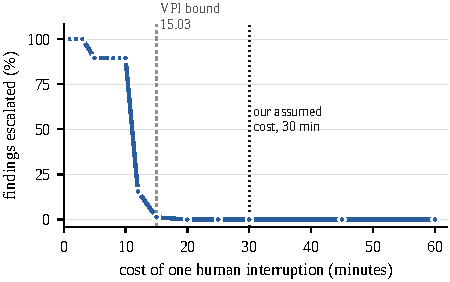
\includegraphics[width=\columnwidth]{figures/escalation.pdf}
\caption{Escalation is a function of one number we guessed. With every other
cost fixed at its point estimate, the agent escalates every finding when a human
costs three minutes and none when a human costs twenty. Our assumed thirty is
well past the crossover; a dedicated triage analyst would not be.}
\label{fig:escalation}
\end{figure}

\begin{figure}[t]
\centering
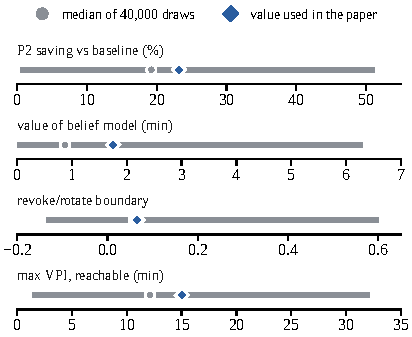
\includegraphics[width=\columnwidth]{figures/intervals.pdf}
\caption{Point estimates against their sampled distributions, 5th to 95th
percentile. Every value we quote sits near the median of its distribution, so
the cost model is not an outlier among plausible ones---but the intervals are
wide enough that quoting any single figure implies a precision the model does
not have. A negative boundary means revoke-now never wins in that world.}
\label{fig:intervals}
\end{figure}

Every point estimate sits near its median, so our cost model is not an outlier
among plausible ones; the intervals are nonetheless very wide. \textbf{The
claims worth keeping are about ordering rather than magnitude.}

\section{Discussion}

Three of this paper's results are negative, and we think that is the point. The
free features cannot separate the states that matter; escalation is not
cost-optimal at our assumed human cost; the probe is usually not worth buying.
Each was established by computation rather than assertion, and each was contrary
to our expectation before it was computed.

The methodological observation we would defend is narrower than an earlier draft
made. Deriving a boundary rather than choosing it does not make the policy
dramatically cheaper---a hand-picked threshold with a sensible fallback beats
the baseline too. What it changes is \textbf{what an objection looks like}. A
tuned threshold can only be defended by authority; a derived one can only be
attacked through a cost, which is a claim a practitioner can correct. One did,
by an order of magnitude. And a derived boundary moves when the world moves,
which is why P2 responds monotonically to the prior where P1 does not.

The result we would most like to see contradicted is
Section~\ref{sec:results}'s: if the belief model is worth $1.75$ minutes, most
of what makes this agent useful is the decision to stop escalating, which
requires no probabilistic machinery. Section~\ref{sec:onecell} shows that rests
on a single estimated cell, and at zero that cell makes the belief model worth
precisely nothing. The finding and its weakest input are the same input.

\section{Limitations}
\label{sec:limitations}

\textbf{The refusal to test the key is ours alone.} Three practitioners advised
calling the provider with the found credential. Every downstream result exists
because of a choice the field does not share.

\textbf{Eight of nine cost components are our estimates.} The ninth was
corrected by practitioners and changed a result, which is the best available
evidence that the other eight are also wrong in unknown directions.

\textbf{The case generator draws from the agent's own likelihood tables}, so the
agent is evaluated in a world that agrees with its assumptions. This flatters
every policy that uses evidence.

\textbf{Actions are atomic; the world is sequential.} Rotate-safely is really
six steps with evidence arriving partway through, and a sequential formulation
would find value for investigation this model cannot see.

\textbf{Rotate-safely is modelled as deterministic remediation.} With
probability $\epsilon$ a rotation silently fails on an undocumented consumer and
the outage is paid anyway; introducing $\epsilon$ makes the revoke/rotate
boundary depend on the outage cost and destroys the invariance of
Section~\ref{sec:results}. A practitioner described exactly this failure.

\textbf{Escalation may be a permission boundary rather than a priced option.} An
agent may lack the authority to revoke another team's credential, which is a
constraint on the action space and not a candidate inside it.

\textbf{The free feature set is not the whole repository.} Repository visibility
and commit semantics would plausibly separate live from revoked;
Section~\ref{sec:robustness} shows that even when they do, the conclusions
barely move.

\textbf{The probe requires a privileged credential.} Reading
\texttt{last\_used\_at} means the scanning pipeline holds an organisation-wide
admin key to triage a single project key---a high-severity credential introduced
to resolve a low-severity finding, and the model prices the minutes without
pricing that asymmetry.

\textbf{A fourth state is known and unmodelled.} A credential that authenticates
but is authorised for nothing---a 403 rather than a 401---is live by our
definition yet carries none of the risk that makes dismissing a live key cost
2400.

\textbf{No live call was made.} No admin credential was held, and the repository
contains no credential material; every string is a synthetic feature descriptor.

\section{Conclusion}

We formulated secret-scanner triage as a decision under uncertainty in which the
hidden state cannot be observed without doing something we are unwilling to do,
and showed the decision is nonetheless tractable because the \emph{costs} are
knowable even when the state is not.

The policy saves $23.2\%$ of modelled engineer-minutes while never escalating.
But the honest headline is smaller and more interesting: a policy observing
nothing at all captures $21.2$ of those points, and joint sensitivity analysis
puts the saving anywhere between $0.5\%$ and $51\%$. In this domain a safe
action that is cheap in every state does most of the work a belief model appears
to be doing---and the contribution of decision theory here is less the posterior
than the discipline of pricing the actions before choosing between them.

\section*{Acknowledgements}

Eight practitioners on \texttt{r/sysadmin} and \texttt{r/devops} answered
questions that changed this work: one repriced the probe by an order of
magnitude, one withdrew an assumption about rotation verifying itself, and one
established that live-versus-revoked is solved for certificates and unsolved for
API keys.

\bibliographystyle{named}
\bibliography{references}

\end{document}
